\documentclass{exam}
\usepackage{listings}
\usepackage{graphicx}

\title{Practical: Introduction to R}
\author{Laura Rodríguez Navas \\ rodrigueznavas@posgrado.uimp.es}
\date{January 2020}

\pagestyle{plain}

\begin{document}
	
	\maketitle

\begin{questions}
    
    \question Generate the numbers 1, 2, ... , 12, and store the result in the vector x.    
    \begin{lstlisting}[language=R, numbersep=0pt, resetmargins=true]
   	x <- c(1:12)
   	x
    \end{lstlisting}
  
    \question Generate four repetitions of the sequence of numbers (6, 2, 4).    
    \begin{lstlisting}[language=R, numbersep=0pt, resetmargins=true]
	s <- c(6, 2, 4)
	rep(s, 4)
    \end{lstlisting}
    
    \question Generate the sequence consisting of six 9s, then five 2s, and finally four 5s. Store the numbers in a 5 by 3 matrix (populating it columnwise).    
    \begin{lstlisting}[language=R, numbersep=0pt, resetmargins=true]
   	s <- c(rep(9, 6), rep(2, 5), rep(5, 4))
   	m <- matrix (s, 5, 3)
   	m
    \end{lstlisting}
    
    \question Generate a vector consisting of 20 numbers generated randomly from a normal distribution. Use the value 100 as seed (in order to be able to replicate the experiments). Setting the seed is done as follows: 
    
    $>$ set.seed(100)
    
    Then, calculate the following statistics about the generated vector: mean, median, variance and the standard deviation. Repeat the generation of the vector and the statistics with and without changing the seed and observe what happens. 
    
    \begin{lstlisting}[language=R, numbersep=0pt, resetmargins=true]
    calculation <- function(v) {
    vmean <- mean(v)
    vmedian <- median(v)
    vvariance <- var(v)
    vdeviation <- sd(v)
    return_list <- list("mean" = vmean, "median" = vmedian, 
    "variance" = vvariance, "deviation" = vdeviation)
    return(return_list)
    }
      
    # with seed    
    set.seed(100)
    v <- rnorm(20)
    values_list_with_seed <- calculation(v)
    print(values_list_with_seed)
    
    
    
    # without seed
    v <- rnorm(20)
    values_list_without_seed <- calculation(v)
    print(values_list_without_seed)
    \end{lstlisting}   
    
    \question From the resources provided with the course, download the file "data1.txt" that contains information about students.
    
    \begin{parts}
    	
        \part Read the data into an R object named students (data is in a space-delimited text file and there is no header row).        
        \begin{lstlisting}[language=R, numbersep=0pt, resetmargins=true]
        students <- read.table("data1.txt", header = FALSE, sep = " ")
        \end{lstlisting}
        
        \part Add the following titles for columns (see section 9):
        height, shoesize, gender, population        
        \begin{lstlisting}[language=R, numbersep=0pt, resetmargins=true]
        names(students) <- c("height", "shoesize", "gender", "population")
        \end{lstlisting}
        
        \part Check that R reads the file correctly. 
               
        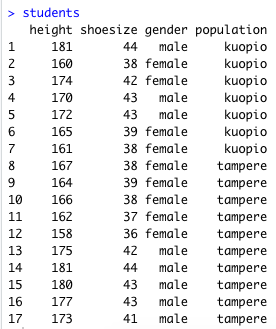
\includegraphics[scale=0.7]{students}
        
        \part Print the header names only.
        \begin{lstlisting}[language=R, numbersep=0pt, resetmargins=true]
        colnames(students)
        \end{lstlisting}
        
        \part Print the column height.
        \begin{lstlisting}[language=R, numbersep=0pt, resetmargins=true]
        students[, 1, drop=FALSE]
        \end{lstlisting}
        
        \part What is the gender distribution (how many observations are in each groups) and the distribution of sampling sites (column population)?
        \begin{lstlisting}[language=R, numbersep=0pt, resetmargins=true]
        summary(students$gender)
       	female male 
       	9      8  
        summary(students$population)
       	kuopio tampere 
       	7      10 
        \end{lstlisting}
        
        \part Show the distributions in the above item at the same time by using a contingency table.
        \begin{lstlisting}[language=R, numbersep=0pt, resetmargins=true]
        table(students$gender, students$population)
	    		kuopio tampere
	    female      4       5
	    male        3       5
        \end{lstlisting}
        
        \part Make two subsets of your dataset by splitting it according to gender.
        Use data frame operations first and then do the same using the function subset. Use the help to understand how subset works.
        
        \part Make two subsets containing individuals below and above the median height. Use data frame operations first and then do the same using the function subset.
        
        \part Change height from centimetres to metres for all rows in the data frame. Do this using in three different ways: with basic primitives, a loop using for and the function apply.
        
        \part Plot height against shoesize, using blue circles for males and magenta crosses for females. Add a legend.
    \end{parts}

\end{questions}

\end{document}